% Created 2020-05-07 jue 11:04
% Intended LaTeX compiler: pdflatex
\documentclass[11pt]{article}
\usepackage[utf8]{inputenc}
\usepackage[T1]{fontenc}
\usepackage{graphicx}
\usepackage{grffile}
\usepackage{longtable}
\usepackage{wrapfig}
\usepackage{rotating}
\usepackage[normalem]{ulem}
\usepackage{amsmath}
\usepackage{textcomp}
\usepackage{amssymb}
\usepackage{capt-of}
\usepackage{hyperref}
\usepackage{minted}
\author{Lucas Michel Todó}
\date{31/03/2020}
\title{Creation of active gene-lists}
\hypersetup{
 pdfauthor={Lucas Michel Todó},
 pdftitle={Creation of active gene-lists},
 pdfkeywords={},
 pdfsubject={},
 pdfcreator={Emacs 26.3 (Org mode 9.2)},
 pdflang={English}}
\begin{document}

\maketitle
\tableofcontents


\section{Active/Inactive Gene lists}
\label{sec:org3f14d4c}
Our aim is to create a unified table that assigns to each gene in the P.falicparum gnome a expresion state.
We will define 4 possible expresion states:
\begin{itemize}
\item Active
\begin{itemize}
\item Regular
\item Variant Active
\item Variant Repressed
\end{itemize}
\item Inactive
\end{itemize}

\subsection{Microarray Data: Red Signal}
\label{sec:org01c354a}
We willl load the red signal and transform it into percentiles. For each gene we pick the "Aver.2Higher" column from the original microarrays data table. This column corresponds to the average between the two highest red signals among available timepoints.

Red Signal DataFrame
\begin{verbatim}
              Gene_id     Red_12B     Red_10G    Red_3D7B Percent_12B
1          mal_mito_3 22579.33333 36436.73333 30636.82500  96.0335622
2 MAL13P1.415_oldname   770.82083   702.22292   640.11667  21.3196034
3  MAL13P1.65_oldname   111.33333    87.05833    91.05833   6.2166285
4  MAL7P1.142_oldname  5924.44167  5194.40000  5114.63333  75.4767353
5  MAL8P1.310_oldname    37.21250    35.37917    33.24167   0.8581236
6   MAL8P1.90_oldname    80.55417    46.18333    54.64167   4.1952708
  Percent_10G Percent_3D7B MaxRedPercentDif
1   98.474447   97.8832952        2.4408848
2   20.861937   18.4591915        2.8604119
3    5.053394    4.5194508        1.6971777
4   72.444699   71.7200610        3.7566743
5    1.115561    0.5911518        0.5244088
6    2.002288    2.2501907        2.1929825
\end{verbatim}

\subsection{Microarray Data: Areas}
\label{sec:org653972a}
We will load the areas data to calculate FC among strains. For each gene, we select the time interval (right, left, mid or sides) for which we find the maximum difference among strains (between highest and lowest). We will also add a column to check if this time interval corresponds to the interval of maxium expression for each strain.

Areas DataFrame
\begin{verbatim}
              Gene_id     l_12B     r_12B     m_12B    s_12B     l_10G    r_10G
1          mal_mito_3 30.592496 61.080128 49.676556 41.99607 25.372470 62.38873
2 MAL13P1.415_oldname  5.423269  8.488971  1.289779 12.62246  6.117132 10.59524
3  MAL13P1.65_oldname 18.322430        NA 17.593468       NA 14.071128       NA
4  MAL7P1.142_oldname  9.389247 12.807814 10.340803 11.85626 13.661078 14.52676
5  MAL8P1.310_oldname        NA        NA        NA       NA        NA       NA
6   MAL8P1.90_oldname        NA        NA        NA       NA        NA       NA
      m_10G    s_10G    l_3D7B   r_3D7B    m_3D7B    s_3D7B   MaxLeft   MinLeft
1 49.805504 37.95570 25.484634 62.83441 50.462696 37.856349 30.592496 25.372470
2  3.676218 13.03616  1.789873 10.51234  3.691753  8.610459  6.117132  1.789873
3        NA       NA 19.333324       NA        NA        NA 19.333324 14.071128
4 13.401610 14.78623  7.099032 13.34518 12.041177  8.403034 13.661078  7.099032
5        NA       NA        NA       NA        NA        NA        NA        NA
6        NA       NA        NA       NA        NA        NA        NA        NA
  MaxRight  MinRight    MaxMid    MinMid MaxSides  MinSides  DifLeft DifRight
1 62.83441 61.080128 50.462696 49.676556 41.99607 37.856349 5.220025 1.754283
2 10.59524  8.488971  3.691753  1.289779 13.03616  8.610459 4.327259 2.106274
3       NA        NA        NA        NA       NA        NA 5.262196       NA
4 14.52676 12.807814 13.401610 10.340803 14.78623  8.403034 6.562046 1.718950
5       NA        NA        NA        NA       NA        NA       NA       NA
6       NA        NA        NA        NA       NA        NA       NA       NA
     DifMid DifSides Interval   MaxDif    areaFC  area_12B area_10G area_3D7B
1 0.7861401 4.139719     Left 5.220025 0.3881060 30.592496 25.37247 25.484634
2 2.4019733 4.425700    Sides 4.425700 0.3290483 12.622460 13.03616  8.610459
3        NA       NA     Left 5.262196 0.3912413 18.322430 14.07113 19.333324
4 3.0608067 6.383199     Left 6.562046 0.4878845  9.389247 13.66108  7.099032
5        NA       NA  No Data       NA        NA        NA       NA        NA
6        NA       NA  No Data       NA        NA        NA       NA        NA
   MaxArea   MinArea
1 30.59250 25.372470
2 13.03616  8.610459
3 19.33332 14.071128
4 13.66108  7.099032
5       NA        NA
6       NA        NA
\end{verbatim}

\subsection{Load RNA-Seq Data}
\label{sec:org8657e6b}
We will use publicly available data from PlasmoDB to create a reference expresion percentile for each gene.
All data-sets are from RNA-Seq studies in the 3D7 strain.
We are using 4 different data-sets:
\begin{itemize}
\item Otto et.al.
\item Hoeijmakers et.al.
\item Toenhake et.al.
\item Bartfai et.al.
\end{itemize}

RNA-Seq DataFrame
\begin{verbatim}
        Gene_id MaxPercOtto MaxPercHoej MaxPercToen MaxPercBart MeanPercent
1 PF3D7_0100100        57.2        54.3        33.9        31.7      44.275
2 PF3D7_0100200        29.4        50.5        26.6        36.0      35.625
3 PF3D7_0100300        34.2         8.7         7.7         7.4      14.500
4 PF3D7_0100400        50.3        18.3        11.3        37.4      29.325
5 PF3D7_0100500        49.7        11.4        14.0        32.5      26.900
6 PF3D7_0100600        18.5         7.8         2.3        12.1      10.175
  StdDevPercent
1     11.546942
2      9.241313
3     11.383980
4     15.424068
5     15.474657
6      5.930167
\end{verbatim}

We plot the standard deviation of the percentile values among different studies and we can see that for the vast majority of genes it doesn't go above 10.
\begin{center}
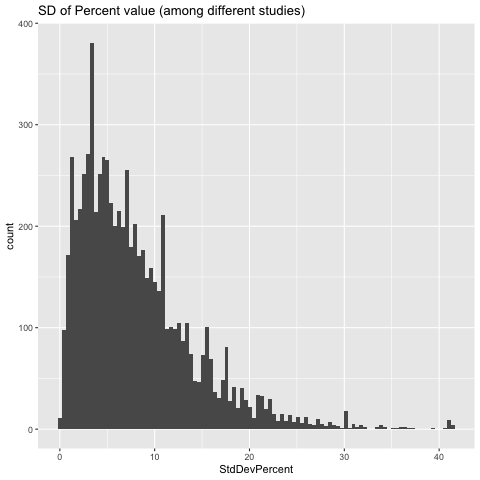
\includegraphics[width=.9\linewidth]{./Plots/rnaseq_perc_sd.png}
\end{center}
\subsection{Create Lists according to thresholds}
\label{sec:org619cff9}

Now that we have all the data loaded in, we can star to set labels for each gene.

We will jhave the following categories:
\begin{itemize}
\item Active : Mean percentile (from rna-seq experiments) >= 25\%
\begin{itemize}
\item Regular : Non-variant according to our variant genes list.
\item Variant Active: Variant according to our variant genes list.
\item Variant Repressed: Variant and red signal percentile differnce > 30\% and area diffrence > 1 (\textasciitilde{}2FC)
\end{itemize}

\item Inactive: Mean percentile (from rna-seq experiments) < 25\%
\end{itemize}

th\_rnapcnt <- 25
th\_redpcnt <- 25
th\_redrescue <- 40
th\_red\_difpcnt <- 0
th\_areaFC <- 1

\section{Code}
\label{sec:org586b077}
Our aim is to create a unified table that assigns to each gene in the P.falicparum gnome a expresion state.
We will define 4 possible expresion states:
\begin{itemize}
\item Active
\begin{itemize}
\item Regular
\item Variant Active
\item Variant Repressed
\end{itemize}
\item Inactive
\end{itemize}

\subsection{Load Packages and functions}
\label{sec:orgac7187e}
\begin{minted}[]{r}
#### Imports ####

library(readxl)
library(tidyverse)

#### Max Dif function ####

max_dif <- function(vect){
  mx <- max(vect, na.rm = T)
  mn <- min(vect, na.rm = T)
  if (is.infinite(mx) | is.infinite(mn)) {
    md <- NA
  } else {
    md <- mx - mn
  }
  return(md)
}
\end{minted}
\subsection{Microarray Data: Red Signal}
\label{sec:org806235c}
We willl load the red signal and transform it into percentiles. For each gene we pick the "Aver.2Higher" column from the original microarrays data table. This column corresponds to the average between the two highest red signals among available timepoints.

\begin{minted}[]{r}
#### Red Signal DF ####

## Read translation table
map <- read.csv('./Data/oldnames_table.csv')
excl <- "./Data/3D7_Variantome_AllData_withGam.xls"

## Import Red Signal table
red <- read_excel(excl, sheet = 4)

colnames(red)[1] <- "Old_id"

red_df <- red %>%
  select(Old_id,
         Red_12B = `Aver.2Higher1.2B.`,
         Red_10G = `Aver.2Higher10G.`,
         Red_3D7B = `Aver.2Higher3D7-B.`) %>%
  left_join(map, by='Old_id') %>%
  select(-Old_id) %>%
  group_by(Gene_id) %>% summarize_all(list(mean))

## Transform into percentiles

red_df <- red_df %>%
  mutate(Percent_12B = (rank(Red_12B)/length(Red_12B))*100) %>%
  mutate(Percent_10G = (rank(Red_10G)/length(Red_10G))*100) %>%
  mutate(Percent_3D7B = (rank(Red_3D7B)/length(Red_3D7B))*100)

## Add max percentile dif

red_df <- red_df %>%
  mutate(MaxRedPercentDif= apply(select(., contains('Percent_')), 1, max_dif))

print(red_df, width = 200)
\end{minted}

Red Signal DataFrame
\begin{minted}[]{r}
head(as.data.frame(red_df))
\end{minted}

\subsection{Microarray Data: Areas}
\label{sec:orge01dae2}
We will load the areas data to calculate FC among strains. For each gene, we select the time interval (right, left, mid or sides) for which we find the maximum difference among strains (between highest and lowest). We will also add a column to check if this time interval corresponds to the interval of maxium expression for each strain.

\begin{minted}[]{r}
#### Areas DF ####

# Import Areas table

area <- read_excel(excl, sheet = 2)

colnames(area)[1] <- "Old_id"

area_df <- area %>%
  select(Old_id,
         l_12B = `left.1.2b`,
         r_12B = `right.1.2b`,
         m_12B = `mid.1.2b`,
         s_12B = `sides.1.2b`,
         l_10G = `left.10g`,
         r_10G = `right.10g`,
         m_10G = `mid.10g`,
         s_10G = `sides.10g`,
         l_3D7B = `left.3d7b`,
         r_3D7B = `right.3d7b`,
         m_3D7B = `mid.3d7b`,
         s_3D7B = `sides.3d7b`) %>%

  mutate_at(vars(-Old_id), as.numeric) %>%


  left_join(map, by='Old_id') %>%
  select(-Old_id) %>%
  group_by(Gene_id) %>% summarize_all(list(mean))


print(area_df, width = 200)

area_df <- area_df %>%
  mutate(MaxLeft = apply(select(., contains('l_')), 1, max)) %>%
  mutate(MinLeft = apply(select(., contains('l_')), 1, min)) %>%

  mutate(MaxRight = apply(select(., contains('r_')), 1, max)) %>%
  mutate(MinRight = apply(select(., contains('r_')), 1, min)) %>%

  mutate(MaxMid = apply(select(., contains('m_')), 1, max)) %>%
  mutate(MinMid = apply(select(., contains('m_')), 1, min)) %>%

  mutate(MaxSides = apply(select(., contains('s_')), 1, max)) %>%
  mutate(MinSides = apply(select(., contains('s_')), 1, min)) %>%

  mutate(DifLeft = MaxLeft - MinLeft) %>%
  mutate(DifRight = MaxRight - MinRight) %>%
  mutate(DifMid = MaxMid - MinMid) %>%
  mutate(DifSides = MaxSides - MinSides)

print(area_df, width = 200)

## Add max interval and difference

maxinterval <- area_df %>%
  select(Gene_id, contains('Dif')) %>%
  pivot_longer(-Gene_id, names_to = 'Interval', values_to = 'MaxDif') %>%
  group_by(Gene_id) %>%
  filter(rank(-MaxDif, ties.method = "first") == 1) %>%
  mutate(Interval = ifelse(is.na(MaxDif), 'No Data', Interval)) %>%
  mutate(Interval = case_when(Interval == 'DifLeft' ~ 'Left',
                              Interval == 'DifRight' ~ 'Right',
                              Interval == 'DifMid' ~ 'Mid',
                              Interval == 'DifSides' ~ 'Sides',
                              Interval == 'No Data' ~ 'No Data')) %>%
  mutate(areaFC = MaxDif/13.45)

maxinterval

area_df <- area_df %>%
  left_join(maxinterval, by = 'Gene_id')

print(area_df, width = 400)

## Select appropiate area for each gene and add max and min areas

area_df <- area_df %>%
  mutate(area_12B = case_when(
           Interval == 'Left' ~ l_12B,
           Interval == 'Right' ~ r_12B,
           Interval == 'Mid' ~ m_12B,
           Interval == 'Sides' ~ s_12B,
           Interval == 'No Data' ~ NA_real_)) %>%
  mutate(area_10G = case_when(
           Interval == 'Left' ~ l_10G,
           Interval == 'Right' ~ r_10G,
           Interval == 'Mid' ~ m_10G,
           Interval == 'Sides' ~ s_10G,
           Interval == 'No Data' ~ NA_real_)) %>%
  mutate(area_3D7B = case_when(
           Interval == 'Left' ~ l_3D7B,
           Interval == 'Right' ~ r_3D7B,
           Interval == 'Mid' ~ m_3D7B,
           Interval == 'Sides' ~ s_3D7B,
           Interval == 'No Data' ~ NA_real_)) %>%
  mutate(MaxArea = apply(select(., contains('area_')), 1, max)) %>%
  mutate(MinArea = apply(select(., contains('area_')), 1, min))


print(area_df, width = 400)
\end{minted}

Areas DataFrame
\begin{minted}[]{r}
head(as.data.frame(area_df))
\end{minted}

\subsection{Load RNA-Seq Data}
\label{sec:orgf9833ca}
We will use publicly available data from PlasmoDB to create a reference expresion percentile for each gene.
All data-sets are from RNA-Seq studies in the 3D7 strain.
We are using 4 different data-sets:
\begin{itemize}
\item Otto et.al.
\item Hoeijmakers et.al.
\item Toenhake et.al.
\item Bartfai et.al.
\end{itemize}

\begin{minted}[]{r}
#### Load Data-Sets ####

otto <- read_delim("./Data/RNA_Seq_Percentiles/PlasmoDB_Otto.csv", delim=";") %>%
  select(Gene_id = `Gene ID`, MaxPercOtto = `Max %ile (Within Chosen Samples)`)
hoej <- read_delim("./Data/RNA_Seq_Percentiles/PlasmoDB_Hoejimakers.csv", delim=";") %>%
  select(Gene_id = `Gene ID`, MaxPercHoej = `Max %ile (Within Chosen Samples)`)
toen <- read_delim("./Data/RNA_Seq_Percentiles/PlasmoDB_Toenke.csv", delim=";") %>%
  select(Gene_id = `Gene ID`, MaxPercToen = `Max %ile (Within Chosen Samples)`)
bart <- read_delim("./Data/RNA_Seq_Percentiles/PlasmoDB_Bartfai.csv", delim=";") %>%
  select(Gene_id = `Gene ID`, MaxPercBart = `Max %ile (Within Chosen Samples)`)

## Join DF
rna_df <- full_join(otto, hoej) %>%
  full_join(hoej) %>%
  full_join(toen) %>%
  full_join(bart)

## Add mean and sd
rna_df <- rna_df %>%
  mutate(MeanPercent = apply(select(., -Gene_id), 1, mean)) %>%
  mutate(StdDevPercent = apply(select(., -Gene_id), 1, sd))


print(rna_df, width=200)
\end{minted}

\begin{minted}[]{r}
head(as.data.frame(rna_df))
\end{minted}

We plot the standard deviation of the percentile values among different studies and we can see that for the vast majority of genes it doesn't go above 10.
\begin{center}
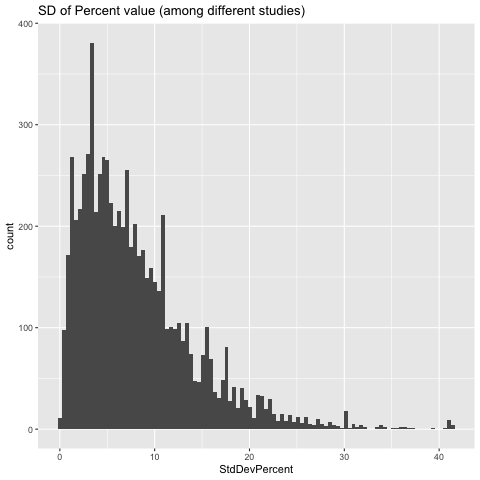
\includegraphics[width=.9\linewidth]{./Plots/rnaseq_perc_sd.png}
\end{center}

\subsection{Create Join DF}
\label{sec:orgbd15704}
\begin{minted}[]{r}
red_df
print(area_df, width = 200)
rna_df

all_df <- select(red_df, Gene_id, contains('Percent')) %>%
  full_join(select(area_df, Gene_id, Interval, contains('area')), by = 'Gene_id') %>%
  full_join(select(rna_df, Gene_id, MeanPercent), by = 'Gene_id')

## Add Vartiant Genes information

cvg <- read_excel("./Data/CVG_list_jan2020_final.xlsx", sheet = "Final")

final_df <- cvg %>%
  select("Gene_id" = `Gene ID`, "Variant" = `Final Customized`) %>%
  right_join(all_df, by = 'Gene_id') %>%
  mutate(Variant = recode(Variant, YES = TRUE, NO = FALSE, .missing = FALSE))

print(final_df, width = 200)
\end{minted}

\subsection{Create Lists according to thresholds}
\label{sec:orgd7a28e3}

Now that we have all the data loaded in, we can star to set labels for each gene.

We will jhave the following categories:
\begin{itemize}
\item Active : Mean percentile (from rna-seq experiments) >= 25\%
\begin{itemize}
\item Regular : Non-variant according to our variant genes list.
\item Variant Active: Variant according to our variant genes list.
\item Variant Repressed: Variant and red signal percentile differnce > 30\% and area diffrence > 1 (\textasciitilde{}2FC)
\end{itemize}

\item Inactive: Mean percentile (from rna-seq experiments) < 25\%
\end{itemize}
\begin{minted}[]{r}
print(final_df, width = 200)

th_rnapcnt <- 25
th_redpcnt <- 25
th_redrescue <- 40
th_red_difpcnt <- 0
th_areaFC <- 1

## Set state for each gene and strain

## Here we create a couple of dplyr functions.
##To be able to use variables (for colnames) we needto use the special quote functions.
## Colnames to use inside functions must be "enquoted" before usage and preceded by !! when used.
## Colnames to assign must be "enquoted" first, preceded by !! and assigned by :=


## First create a col where we set categories for each gene according relative expression
## For each gene: gene-min----|---mid----|----gene-max

relexprs <- function(vect){
  if (any(is.na(vect))){
    return(NA)
  } else {
    labs = c('min', 'mid', 'max')
    lab <- cut(vect, 3, labels = labs)[1]
    return(as.character(lab))
  }
}

set_relexprs <- function(df, outcol, areacol){
  outcol <- enquo(outcol)
  areacol <- enquo(areacol)
  df %>%
    mutate(!! outcol := apply(select(., !! areacol, MaxArea, MinArea), 1, relexprs))
}

final_df <- final_df %>%
  set_relexprs(rel_12B, area_12B) %>%
  set_relexprs(rel_10G, area_10G) %>%
  set_relexprs(rel_3D7B, area_3D7B)

print(final_df, width = 200)

## We now set each gene to it's state
set_state <- function(df, statecol, redcol, relcol){

  statecol <- enquo(statecol)
  redcol <- enquo(redcol)
  relcol <- enquo(relcol)

  df <- df %>%
    mutate(!! statecol := case_when(
                ## Actiu
                !Variant & MeanPercent >= th_rnapcnt ~ 'Active',
                ## Inactiu
                !Variant & MeanPercent < th_rnapcnt ~ 'Inactive',

                ## Var actiu
                Variant &
                areaFC < th_areaFC &
                MeanPercent >= th_rnapcnt ~ 'Var_Active', # noFC

                Variant &
                areaFC < th_areaFC &
                MeanPercent < th_rnapcnt &
                !! redcol >= th_redrescue ~ 'Var_Active', # noFC, rescued

                Variant &
                areaFC >= th_areaFC &
                MaxRedPercentDif >= th_red_difpcnt &
                !! redcol >= th_redpcnt &
                !! relcol == 'max' ~ 'Var_Active', # Variant, FC, redpcnt, max

                Variant &
                areaFC >= th_areaFC &
                MaxRedPercentDif >= th_red_difpcnt &
                !! redcol >= th_redpcnt &
                !! relcol == 'mid' ~ 'Var_Semiactive', # Variant, FC, redpcnt, mid

                ## Var repressed
                Variant &
                areaFC < th_areaFC &
                MeanPercent < th_rnapcnt &
                !! redcol < th_redrescue ~ 'Var_Repressed', # noFC, noRescued

                Variant &
                areaFC >= th_areaFC &
                MaxRedPercentDif >= th_red_difpcnt &
                !! redcol >= th_redpcnt &
                !! relcol == 'min' ~ 'Var_Repressed', # Variant, FC, redpcnt, min

                Variant &
                areaFC >= th_areaFC &
                MaxRedPercentDif >= th_red_difpcnt &
                !! redcol < th_redpcnt ~ 'Var_Repressed', # Variant, FC, NOredpcnt

                ## Not settable
                is.na(areaFC) | is.na(MeanPercent) ~ 'Not_settable',

                TRUE ~ 'Wrong!'))
  return(df)
}


state_df <- final_df %>%
  set_state(state_12B, Percent_12B, rel_12B) %>%
  set_state(state_10G, Percent_10G, rel_10G) %>%
  set_state(state_3D7B, Percent_3D7B, rel_3D7B)


state_df %>%
  filter(state_12B == 'Wrong!' | state_10G == 'Wrong!' | state_3D7B == 'Wrong!') %>%
  print(width = 200)

## The 'TRUE ~ ...' handles rows that do not match any of previous patterns.
## Here we use it to make sure all rows are set (no "Wrong!" appearing)

table(state_df$state_3D7B)
table(state_df$state_12B)
table(state_df$state_10G)

write.csv(state_df, './Results_Tables/state_df_rna25_red25_reddif0_area1.csv')

print(state_df, width = 200)

state_df %>%
  filter(state_12B != state_10G) %>%
  select(contains('12B'), contains('10G')) %>%
  write.csv('./Results_Tables/gens_dif12B_10G.csv')


state_df %>%
  filter(Gene_id == 'PF3D7_0302500' | Gene_id == 'PF3D7_0302200') %>%
  write.csv('./Results_Tables/clag_genes.csv')
\end{minted}
\end{document}
